\section{Поиск $\Lambda_c$}
\label{Lamc:search}
\subsection{Критерии отбора}
На основе выбранных нами каналов $X_c$, описанных в предыдущем разделе, 
отбираются события, удовлетворяющие условию:

\begin{equation}
    \abs{p_{e^+} + p_{e^-} - p_{X_c}}^2 \leq 3 \ \text{GeV}^2
\end{equation}

В идеальных условиях это выражение должно быть равно квадрату массы $\Lambda_c$, 
$M^{\text{real}}_{\Lambda_c} = 2226.46 \ \text{MeV}$. Таким образом, данное ограничение позволяет исключить множество событий, соответствующих возбужденным состояниям $\Lambda_c$ или содержащих ошибки в восстановлении треков.

Для отобранных событий осуществляется сборка $\Lambda_c$ барионов по каналам 
$\Lambda_c^+ \to \Lambda \pi^+$, $\Lambda_c^+ \to \Lambda \nu_e e^+$ и $\Lambda_c^+ \to \Lambda \nu_\mu \mu^+$.

\newdot Для отбора $e^\pm$ требуем $p_{e^\pm} \geq 0.6 \ \text{GeV}$, чтобы частицы достигли внутреннего детектора SVD, где они участвуют в электронно-фотонном каскаде $e^- \to \gamma e^- \to 2e^- e^+$. Это позволяет эффективно идентифицировать электроны, поэтому критерий на $L(e) > 0.1$ не является строгим.

\newdot Для отбора $\mu^\pm$ также требуем $p_{\mu^\pm} \geq 0.6 \ \text{GeV}$, чтобы они достигли детектора KLM, где их идентификация ещё более надёжна. Требуется $L(\mu) > 0.01$.

\newdot Для отбора $\Lambda \to p \pi$ предъявляются следующие требования:

$$
\abs{ M_{\Lambda} - M^{\text{real}}_{\Lambda} } < 30 \ \text{MeV}; 
\ \rho_{\Lambda} > 1 \ \text{mm}; \ z_{\Lambda} > 1 \ \text{cm}; 
\ \cos \theta_{\Lambda} > 0.99.
$$

\newdot Комбинируем $\Lambda_c$ с массовым окном $50 \ \text{MeV}$.

\newdot Независимо от \cite{BelleDetector2002}, среди множества идентифицированных дочерних продуктов распада частицы $\xi$ можно использовать известные свойства импульсов этих продуктов, исходящих из вершины распада, для корректировки измеренных импульсов. Это позволяет улучшить точность, соответствуя гипотезе (далее этот метод будет называться "фитом в вершину"). Аналогично, исходя из известной инвариантной массы для $\xi$, импульсы дочерних частиц могут быть скорректированы так, чтобы $M_p = \sqrt{\sum_n \inner{p_n}_\gamma \inner{p_n}^\gamma}$ совпадала с $M^{\text{real}}_{\xi}$, где $p_n$ — 4-импульс, соответствующий $d_n$. Этот метод будет называться "фитом в массу". Для этих целей использованы алгоритмы фита в вершину и массу, принятые в коллаборации KEK и описанные в \cite{Krohn2021}.

Итоговая процедура включает фиты в вершину, а затем в массу для всех собранных частиц: $\Lambda_c, D^{\pm}, D^0, D^{*\pm}, D^{*0}, \Lambda, K_s^0$.

\newdot Импульс $X_c$ фитируется таким образом, чтобы $\abs{p_{e^+} + p_{e^-} - p_{X_c}}^2 = M^2_{\Lambda_c}$, что подробно описано в приложении \ref{fit_rec_mass}.

\subsection{Результаты отбора}

В результате отбора было получено $3846$ событий в канале $\Lambda \pi$ и $5149$ --- в канале $\Lambda_c \to \Lambda \ell \nu_\ell$. Однако среди событий всё ещё остаётся множество неправильно идентифицированных случаев (например, $X_c \to D^{*0} p \to D^0 \pi^0 p$ и $X_c \to D^0 \pi^0 p$ могут быть перепутаны, так как в восстановлении участвуют одинаковые частицы), либо могут быть утеряны треки (например, в случае $\pi \to \gamma \gamma$ возможна потеря одного фотона). Поэтому перед анализом данных будет проведён дополнительный отбор лучших кандидатов, который описан в следующем разделе. 

\begin{figure}[H]
    \centering
    \begin{minipage}[b]{0.48\linewidth}
        \centering
        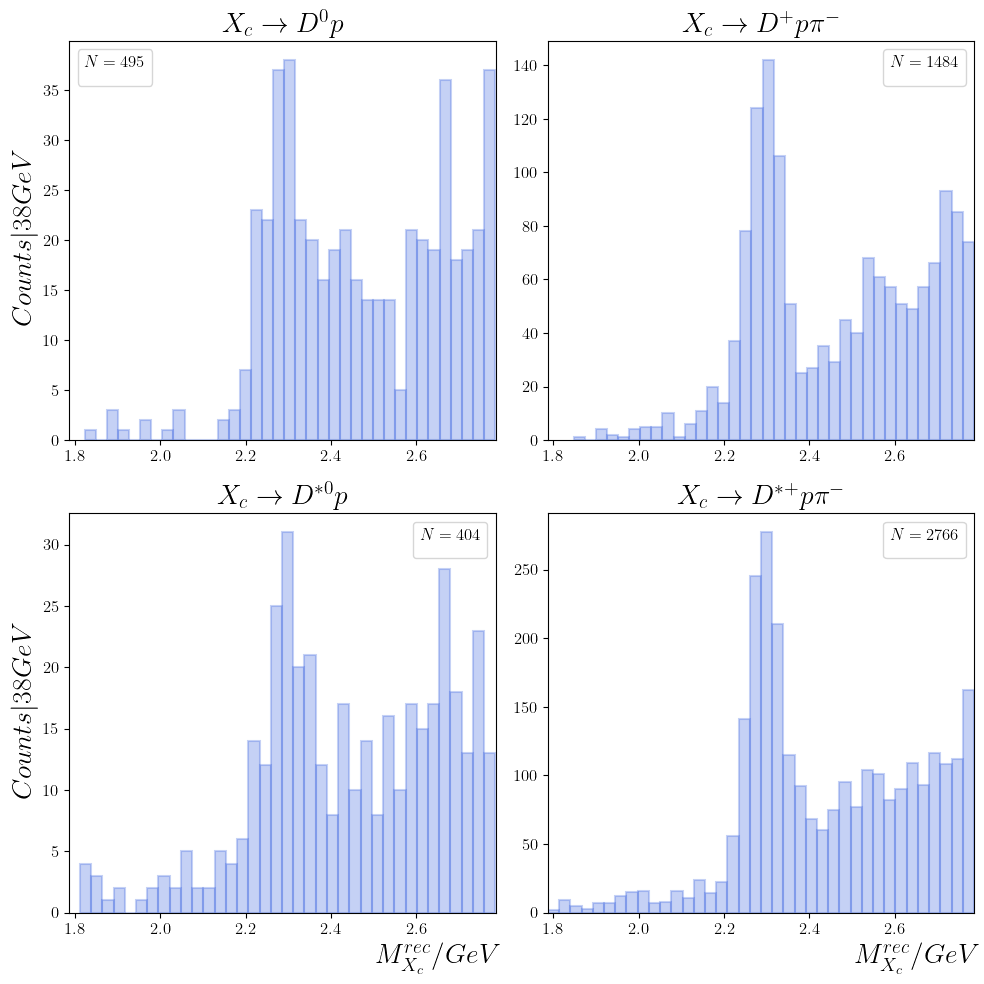
\includegraphics[width=\linewidth]{img/lc_l_nu.png}
        \caption{Распределение отобранных событий по восстановленной массе $\Lambda_c$ до фита для канала $\Lambda_c \to \Lambda \ell \nu_\ell$.}
    \end{minipage}%
    \hfill
    \begin{minipage}[b]{0.48\linewidth}
        \centering
        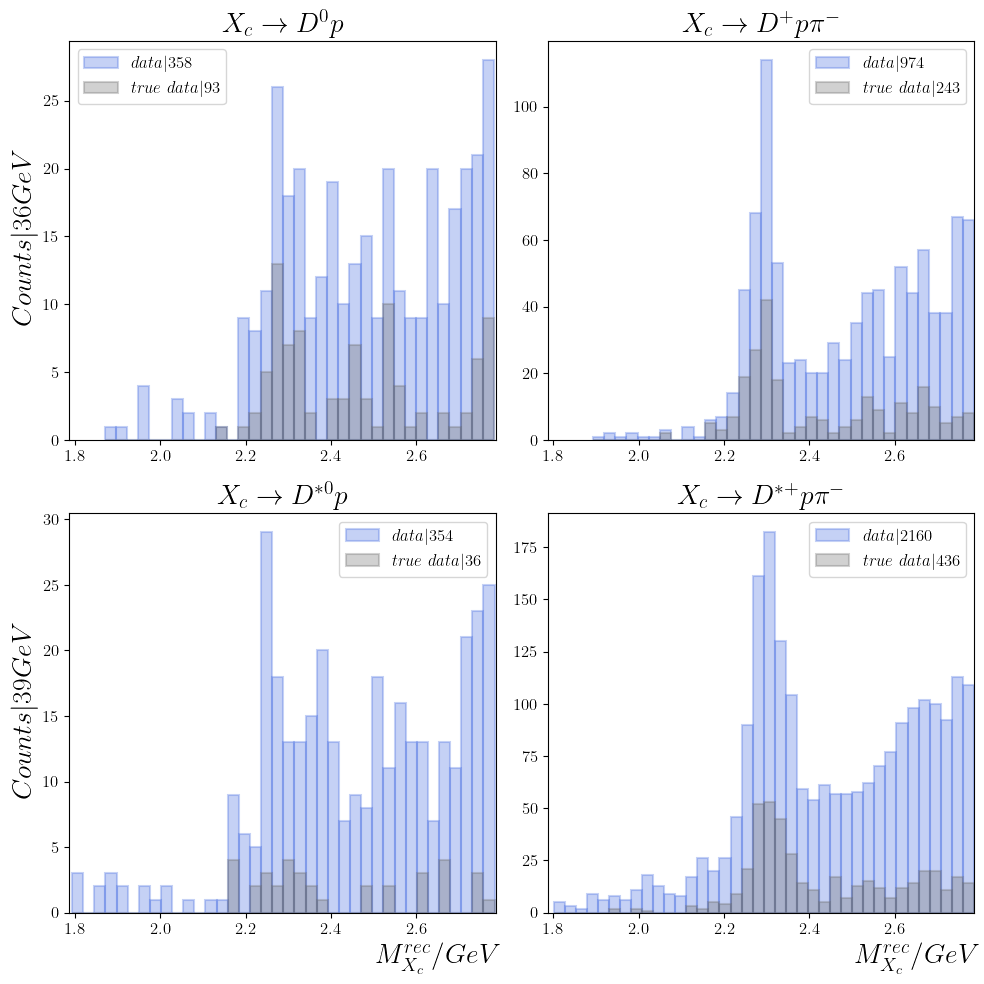
\includegraphics[width=\linewidth]{img/lc_pi.png}
        \caption{Распределение отобранных событий по восстановленной массе $\Lambda_c$ до фита для канала $\Lambda_c \to \Lambda \pi$.}
    \end{minipage}
\end{figure}



